\documentclass[a5paper]{article}
\usepackage[a5paper, top=17mm, bottom=17mm, left=17mm, right=17mm]{geometry}
\usepackage[utf8]{inputenc}
\usepackage[T2A,T1]{fontenc}
\usepackage[colorlinks,filecolor=blue,citecolor=green,unicode,pdftex]{hyperref}
\usepackage{cmap}
\usepackage[english,russian]{babel}
\usepackage{amsmath}
\usepackage{amssymb,amsfonts,textcomp}
\usepackage{color}
\usepackage{array}
\usepackage{hhline}
\hypersetup{colorlinks=true, linkcolor=blue, citecolor=blue, filecolor=blue, urlcolor=blue, pdftitle=1, pdfauthor=, pdfsubject=, pdfkeywords=}
\usepackage[pdftex]{graphicx}
\usepackage{graphicx}
%\usepackage{literat}
\usepackage{indentfirst}
\usepackage{multirow}
\usepackage{subfig}

\sloppy
\pagestyle{plain}

\title{Подходы к заданию семантики интерпретации диаграмм в рамках DSM-подхода}

\author{В.А.Поляков \and Т.А.Брыксин}
\date{}
\begin{document}

\maketitle
\thispagestyle{empty}

\begin{quote}
\small\noindent
В статье рассматривается задача интерпретации визуальных языков моделирования. Приводится обзор основных способов описания семантики визуальных языков, необходимой для осуществления такой интерпретации. Анализируются следующие подходы: двухуровневая схема отладки, Executable UML, EProvide и Dynamic Meta Modeling. Делаются выводы о применимости данных подходов при разработке DSM-платформ.
\end{quote}

\section*{Введение}

В настоящее время большинство уже существующих и разрабатываемых технологий программирования основано на текстовых языках. Для таких текстовых языков есть много интегрированных сред разработки и других программных продуктов, значительно повышающих удобство и скорость создания новых программ. Каждый из этих продуктов предоставляет широкий набор различной функциональности, позволяющей разработчику программировать более эффективно. Одной из них является возможность пошаговой интерпретации и/или отладки написанного кода.

Помимо текстовых языков при разработке ПО в последнее время часто используется модельно-ориентированные средства разработки (model-based development). Этот подход предназначен для описания самой системы и ее предметной области в виде множества моделей, характеризующих её с разных сторон. При этом часто даже создаются новые специализированные предметно-ориентированные языки (DSL), хорошо подходящие под конкретные задачи, и эти задачи решаются уже с их помощью. При наличии такого нового специализированного языка скорость решения поставленных задач может существенно возрастать, модели становятся более наглядными и понятными, оказывается возможной эффективная автоматическая кодогенерация из них. Такой подход к разработке ПО называют предметно-ориентированным моделированием~\cite{koznov1, koznov2, koznov4, koznov6, dsmbook}.

Существует множество визуальных сред разработки, обзор таких средств можно найти в~\cite{koznov3, koznov5}. Один из способов сделать эти средства более удобными --- заимствовать привычную и хорошо зарекомендовавшую себя функциональность, например, подсветку синтаксиса, автодополнение, автоматический рефакторинг и т.п. из аналогичных инструментов для текстовых языков. Распространение возможности пошаговой интерпретации и отладки на поведенческие визуальные модели является одним из шагов по достижению этой цели. Подобный инструмент позволяет разработчику искать и исправлять ошибки на ранних этапах разработки. Также визуальная интерпретация диаграмм способствует лучшему пониманию проектировщиком принципов работы разрабатываемой системы, что, в итоге, повышает её качество.

В некоторых UML-пакетах (например, в Borland Together\footnote{Borland Together, \url{http://www.borland.com/products/Together}}) возможность визуальной интерпретации и отладки уже присутствует. Однако данный подход было бы полезно распространить и на DSM-платформы, с помощью которых можно создавать и реализовывать новые DSL и соответствующие им DSM-пакеты. Это позволит пользователю таких систем быстро создавать интерпретаторы и отладчики для разрабатываемых им визуальных языков. Для создания подобных интерпретаторов необходимо задать формальную семантику для элементов соответствующего визуального языка. Цель данной статьи --- дать обзор основных способов спецификации этой семантики, сделать выводы относительно их применимости и возможности улучшения. В работе рассматриваются следующие подходы: двухуровневая схема отладки, Executable UML, EProvide и Dynamic Meta Modeling. 

\section{Семантика языков}

Любой новый язык является набором знаков, при помощи которых пользователь, следуя определенным правилам, может составить некий текст. Традиционно любой язык раскладывается по трём измерениям: синтаксис, определяющий правила построения текстов из знаков, семантика, задающая проекции знаков на предметную область языка, и прагматика, описывающая способы использования языка пользователем.

Для языков визуального моделирования выделяют три вида синтаксиса: абстрактный, конкретный и служебный. Служебный синтаксис отвечает за представление визуальных спецификаций на данном языке в памяти. Абстрактный синтаксис определяет набор правил, при помощи которых можно объединять простые составляющие языка (знаки и конструкции) в сложные (тексты, т.е. визуальные модели). Обычно он задаётся в виде грамматики или метамодели. Конкретный синтаксис (графическая нотация или просто нотация) состоит из формализованного набора графических символов, которыми пользователь может записывать тексты, т.е. из правил изображения конструкций языка. Семантика позволяет же придавать конструкциям смысл, т.е. определяет их соответствие реальным ситуациям из предметной или из любой другой формально определённой области, называемой семантической областью. Например, семантика интерпретации используется для преобразования абстрактного представления этих конструкций в исполнимое.

В теории языков программирования выделяют четыре основных типа семантик: операционная, денотационная, аксиоматическая и трансляционная.

Денотационная семантика была описана в работе~\cite{semantics2}. Обычно при таком подходе в качестве семантической области используются некоторые математические объекты или функции, называемые денотациями (denotation), а соответствие конструкций языка этим объектам задаётся рекурсивно, т.е. денотация для выражения должна составляться из денотаций подвыражений. Часто это соответствие задаётся при помощи $\lambda$-исчисления. Данный тип семантик является математически строгим и формальным, но в чистом виде порой не обладает достаточной степенью понятности для неспециалистов.

Операционная семантика\footnote{\url{http://en.wikipedia.org/wiki/Operational_semantics}} также является математически строгой и бывает двух типов: структурная операционная семантика (семантика малого шага,~\cite{semantics1}) и естественная семантика (семантика большого шага,~\cite{plotkin}).  Структурная операционная семантика состоит из набора правил, при помощи которых исполнение конкретной программы на данном языке будет представлено в виде последовательности индивидуальных вычислительных шагов. После применения этих правил могут оставаться некоторые остаточные вычисления, учитывающиеся при дальнейшем представлении программы в виде набора вычислительных шагов. Естественная семантика такие остаточные вычисления запрещает и сразу определяет, каким образом по выражению будет получен конечный результат.

Аксиоматические семантики~\cite{hoare} представляют собой набор логических аксиом. Для них любые выражения, записанные на данном языке, рассматриваются в виде логических формул, значение которых будет формально выведено из исходного набора аксиом.

Ещё одним важным типом семантик являются трансляционные~\cite{translational}. Они состоят из набора правил преобразования моделей, с помощью которых модель на исходном языке переводится в модель на другом языке, для которого уже задана семантика исполнения. Например, часто это сводится к генерации кода на языке общего назначения, для которых существуют компиляторы и отладчики (Java, C++, Python и т.п.). Такой подход, с одной стороны, требует от разработчика знаний сразу в обеих областях (исходной и целевой), а с другой --- является хорошо воспринимаемым, т.к. понятия абстрактной исходной предметной области переходят в конкретные конструкции исполнимого языка.

Приведя основные общие типы задания семантики языков программирования, перейдём к рассмотрению ряда конкретных подходов, предложенных в различных работах и использующихся в программных средствах.

\section{Двухуровневая схема отладки}

Наиболее интуитивным с точки зрения реализации способом задания семантики исполнения языков является непосредственное создание интерпретатора или отладчика для конкретного предметного языка в виде отдельного модуля. Работает данный модуль по следующему принципу. По модели генерируется машинный код, который затем интепретируется, а процесс исполнения отслеживается и определённым образом отображается пользователю. Также очевидна проекция стандартного функционала отладчиков на такую систему. Наличие машинного кода позволяет осуществлять пошаговую интерпретацию, ставить точки останова, следить за хранящимися данными.

Но бывают ситуации, когда применение данного подхода либо совершенно неэффективно, либо вообще невозможно, например, в случае языков со сложными проекциями типов данных и операторов. Такими языками в том числе являются и визуальные языки. Сложности могут возникать как и при самой генерации машинного кода, так и при организации отслеживания хода исполнения. Поэтому Карташев в своей статье~\cite{kartashev} предлагает реализовывать отладчики для таких языков по двухуровневой схеме, т.е. при помощи генерации кода на объектном языке и использования существующего отладчика этого языка.

\subsection{Описание}

Двухуровневая схема отладки основана на идее двухуровневой трансляции, которая состоит в том, что программа на исходном языке транслируется в программу на другом, целевом языке, для которого существуют компилятор и отладчик.

Если посмотреть на процесс отладки со стороны исходного языка, то он должен происходить в терминах этого исходного языка, т.е. положение потока исполнения в исходном коде, точки останова в определённых местах исходного кода и др. Поэтому, например, команда пошаговой отладки с остановкой на том же уровне стека вызовов (step over) должна учитывать изменение стека вызовов исходной программы, а не объектной. Сам же стек вызовов исходной программы лишь конструируется на основе стека вызовов объектной программы.

Более подробно данную проблему можно описать на примере следующим образом. По коду программы на исходном языке генерируется код на некотором объектном языке, и установка точек останова происходит в нём в терминах номеров строк кода. Каждой конструкции программы на исходном языке соответствует несколько строк кода на объектном, поэтому для того, чтобы установить точку останова в терминах исходного языка, необходимо знать, на какую из этих строк кода нужно ставить точку останова в объектном языке. Также это нужно учитывать и при простой пошаговой отладке, т.к. не всегда переход к следующему элементу потока исполнения в исходной программе будет соответствовать переходу на следующую строку кода в объектном.

Таким образом, создание отладчика исходного языка нужно производить на основе существующего отладчика объектного языка. Этот отладчик должен иметь интерфейс доступа к таким функциям, как запуск, приостановка и принудительное завершение программы, установка и снятие точек останова в терминах объектного языка, получение информации о стеках потоков вызовов в программе и др. В статье~\cite{kartashev} приведено описание того, как данные стандартные функции могут быть реализованы в терминах исходного языка.

\subsection{Анализ}

Несмотря на понятную идею в плане реализации, данный подход требует от разработчиков новых предметных языков серьезных инженерных навыков для организации точного и полного соответствия конструкций исходного языка конструкциям целевого объектного языка и взаимодействия этих конструкций. 

В связи с высокой технической сложностью задачи и тем, что данный подход ориентирован на создание единичного отладчика для определённого языка, обобщение подхода двухуровневой отладки на предметно-ориентированное моделирование выглядит нецелесообразным. Для нового языка процесс нужно будет повторять заново со всеми техническими деталями, что не дает существенного упрощения, ускорения и автоматизации процесса создания отладчика по сравнению с ручным кодированием.

\section{xUML}

Появление унифицированного языка моделирования UML (Unified Modeling Language)~\cite{uml} и его использование для объектно-ориентированного моделирования при разработке ПО способствовало сильному продвижению визуального проектирования среди разработчиков. Однако, сам по себе UML --- это язык именно проектирования и документирования, а не программирования, семантика многих его элементов либо не задана явно, либо чересчур детально, но не формально описана в спецификации, благодаря чему могут случаться различные ошибки в их согласованности. Для того чтобы применять диаграммы UML для генерации кода, был создан язык, получивший название исполняемого UML (Executable UML, xUML~\cite{xuml1, xuml2, xuml3}). Формально этот язык является профилем UML, т.е. подмножеством языка UML c четко определённой семантикой для каждого элемента. Это подмножество выбрано так, чтобы сделать на основе UML полноценный визуальный язык программирования общего назначения. Также как и UML, xUML основан на объектно-ориентированном подходе,
 т.
е. описание системы ведется в терминах классов, атрибутов и т.п.

\subsection{Задание семантики при помощи xUML}

Для задания семантики отдельных элементов в xUML используется явно определённая семантика действий (Precise Action Semantics, PAS\footnote{Стандартизирована Object Management Group (OMG) в 2001 году}~\cite{xuml3}). PAS --- это фиксированный набор семантических операций, не имеющий конкретного синтаксиса и реализации. PAS обеспечивает независимость, например, от конкретной целевой платформы или языка, на которых будут исполняться модели. Благодаря тому, что элементы обладают фиксированной семантикой, появляется возможность однозначно генерировать исполняемый код по модели, т.е. можно говорить об интерпретации модели.

Программирование на  xUML основано на трёх следующих компонентах.
\begin{itemize}
 \item Диаграмма классов, характеризующая структурную модель наблюдаемой системы. В неё входит отображение объектов реального мира классами. Эти классы имеют атрибуты, а связи между классами представляются в виде отношений.
 \item Диаграмма состояний, определяющая набор действий, которые совершит активный объект, т.е. изображающая жизненный цикл объекта, представленный в виде конечного автомата.
 \item Язык действий (Action Language, AL), позволяющий задавать поведение объекта при проходе каждого состояния в диаграмме состояний. Он необходим для создания экземпляров классов, установки связей между ними, выполнения различных операций над атрибутами и т.п. AL является конкретной реализацией PAS, выбор которой лежит на пользователе, а не заложен в xUML. xUML явно определяет только PAS.
\end{itemize}

Таким образом, упрощенно данный подход основан на представлении поведения системы в виде набора диаграмм состояний для каждого активного объекта. Действия при проходе каждого состояния в таких диаграммах записываются при помощи AL.

В качестве примера на рис.~\ref{fig1} изображён фрагмент полной структуры исполняемой модели в xUML для задачи автоматизации системы контроля поездов. Среди главных доменов (domains) этой предметной области можно выделить следующие: непосредственное управление поездами (train management) и аппаратный интерфейс (hardware interface) всей системы.

В рамках области управления поездами можно выделить две основные сущности (Classes): поезд (Train) и поездка (Hop). Каждая поездка была осуществлена (is being made by) ровно одним поездом, и могут существовать поезда, которые ещё никуда не ездили (is making). Поездку характеризуют начальная дата (атрибут startDate) и время (атрибут startTime), покрытое расстояние (атрибут distanceCovered) и текущее состояние (атрибут currentState), завершилась она или нет. Также у неё есть один метод reportDistanceCovered, который позволяет узнать, чему равно покрытое расстояние. Поезд же характеризуется своей текущей скоростью (атрибут currentSpeed), состоянием (атрибут currentState) и таймером (атрибут timerId).

\begin{figure} [ht]
  \begin{center}
    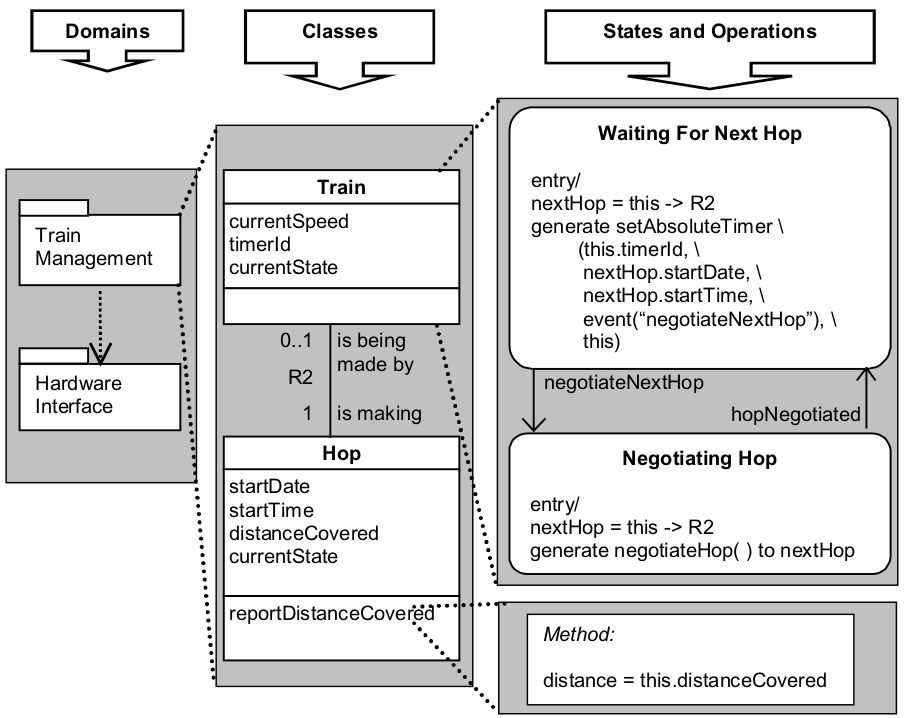
\includegraphics[width=0.9\textwidth]{xuml-example.png}
    \caption{Пример описания системы в xUML (рисунок взят из~\cite{xuml4})}
    \label{fig1}
  \end{center}
\end{figure}

Описание диаграмм состояний и операций для данных классов (States and operations) выполнено с помощью языка действий ASL~\cite{al2}. Метод reportDistanceCovered выдаёт нужное значение и в комментариях не нуждается. Диаграмма состояний для поезда также довольно проста. На ней показано всего два состояния: ожидание следующей поездки (waiting for the next hop) и инициализация новой (negotiating hop). При ожидании новой поездки происходит следующее: из отношения R2 между поездом и  поездкой, описанного на уровне классов, выбирается следующая поездка, после этого выставляется таймер возбуждения события negotiateNextHop, переводящий поезд во второе состояние, на начальное время поездки nextHop. В состоянии инициализации новой поездки её значение опять берётся из отношения R2, и после этого вызывается метод negotiateHop для данной поездки. Его завершение означает конец поездки, и по событию hopNegotiated поезд возвращается в первое состояние.

Действие и PAS  --- это ключевые понятия в исполняемой части языка xUML. Действие — это конкретная операция, определённая на элементе модели, принадлежащая классу и характеризующая его поведение после инициализации. Достаточно выучить только один AL, т.к. остальные будут иметь тот же семантический набор операций. На данный момент существует довольно много готовых AL: OAL~\cite{oal}, SMALL~\cite{al1}, TALL~\cite{xuml3} и т.д.

Пример использования языка действий можно увидеть на рис.~\ref{fig2}. Этот код по своей структуре и внешнему виду похож на обычное текстовое описание и мало напоминает текст на обычном языке программирования.

\begin{figure} [ht]
  \begin{center}
    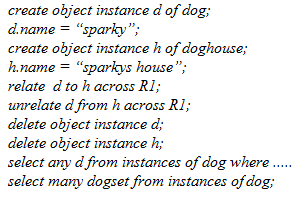
\includegraphics[width=0.5\textwidth]{xuml-oal-syntax.png}
    \caption{Пример описания действий на языке OAL (рисунок взят из работы~\cite{xuml2})}
    \label{fig2}
  \end{center}
\end{figure}

В данном примере показано следующее. Сначала создаётся (create object instance) объект d класса dog, т.е. в систему добавляется ещё одна собака. Ей даётся имя “sparky” присваиванием атрибуту name объекта d соответствующего значения. Дальше аналогично создается собачья будка h класса doghouse с именем “sparkys house”. Затем они сначала связываются (relate d to h) при помощи отношения R1 (across R1), а потом эта связь убирается (unrelate d from h across R1). Объекты d и h удаляются из памяти при помощи оператора delete object instance. В конце приведён пример того, как можно делать различные выборки среди всех объектов, присутствующих в системе. Оператор select any выбирает любой инициалированный объект указанного класса, удовлетворяющий условию, находящемуся в блоке where, который может отсутствовать. В рамках примера ищется произвольная собака d класса dog, удовлетворяющая некоторому условию. При помощи select many можно получить всё множество удовлетворяющих условию объектов класса. В примере после 
выполнения select many переменная dogset будет содержать все объекты класса dog.

\subsection{Анализ}

Существует несколько программных средств (например, CASSANDRA/xUML\footnote{CASSANDRA/xUML, \url{http://www.knowgravity.com/ger/value/cassandra.htm}}, Cameo Simulation Toolkit\footnote{Cameo Simulation Toolkit, \url{http://www.magicdraw.com/simulation}}, Telelogic Tau\footnote{Telelogic Tau, \url{http://www-01.ibm.com/software/awdtools/tau/}}, UniMod\footnote{UniMod, \url{http://unimod.sourceforge.net/index.html}}~\cite{unimod}), позволяющих интерпретировать диаграммы на xUML. Однако, этот язык основан на понятиях объектно-ориентированного подхода и на стандартных конструкциях текстовых языков программирования (ветвления, циклы и т.п.), поэтому на практике значительного повышения уровня абстракции он не даёт. Поведение системы нужно описывать в терминах диаграмм состояний, хотя в общих случаях оно может быть устроено так, что его выражение при помощи конечных автоматов будет очень громоздким и сложным.

\section{Dynamic Meta Modeling}

Другим интересным способом задания семантики визуальных языков является Dynamic Meta Modeling (далее DMM). Этот подход подробно рассмотрен в кандидатской диссертации Яна Хаусмана (Jan Hausmann) из университета в Падерборне (Германия)~\cite{dmm2}. Несмотря на то, что приведённое в работе исследование изложено с опорой на UML, DMM позволяет определять семантику для любых визуальных языков. DMM обладает высокой степенью формальности, ясен и адекватен при определении семантики интерпретации визуальных языков и основывается на концепции семантики действий (action semantics), совместившей в себе черты как денотационной, так и операционной семантики.

\subsection{Описание}

Общая схема DMM-подхода изображена на рис.~\ref{fig3}. Данный рисунок построен, исходя из предположения, что абстрактный язык программирования должен состоять из трёх частей: описания синтаксиса (syntax definition), описания семантики (semantics definition, т.е. множества возможных действий) и семантического соответствия (semantic mapping), которое отвечает за придание определённым синтаксическим конструкциям некого семантического смысла.

\begin{figure} [ht]
  \begin{center}
    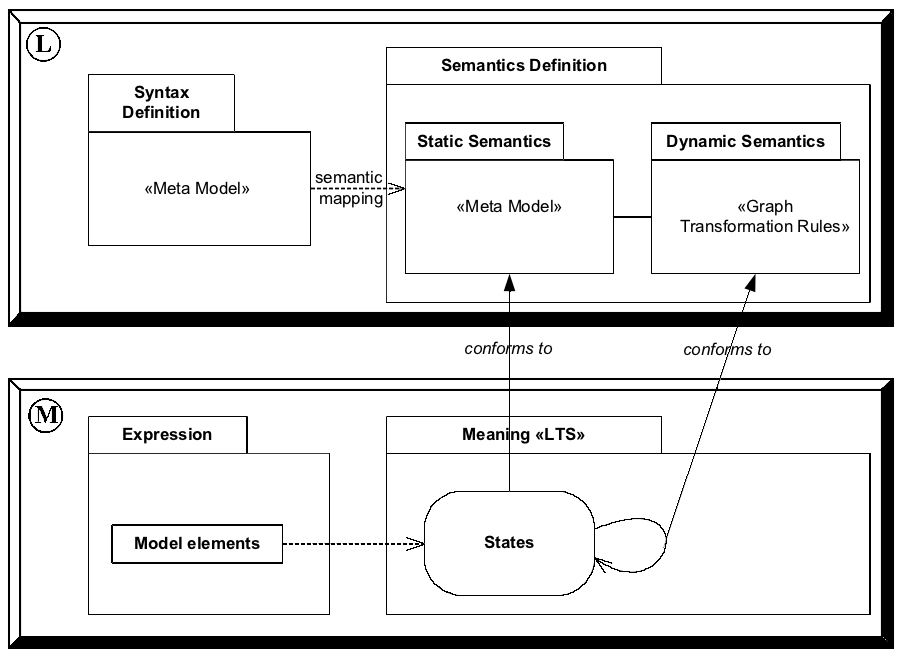
\includegraphics[width=0.9\textwidth]{dmm-concept.png}
    \caption{Общая схема DMM-подхода (этот рисунок и все последующие в этом разделе взяты из работы~\cite{dmm2})}
    \label{fig3}
  \end{center}
\end{figure}

Для всех визуальных языков характерно наличие двух уровней: уровня языка и уровня модели (в литературе также встречаются другие термины --- уровень метамодели и уровень модели соответственно). Уровень языка содержит описание синтаксиса языка, правила отрисовки графических элементов и описание других его особенностей. На уровне модели происходит непосредственное создание конкретной спецификации (expression) на этом языке, состоящей из элементов метамодели (model elements). На рис.~\ref{fig3} эти уровни помечены буквами “L” (language) и “M” (model). Наличие такого разделения подразумевает, что компоненты на уровне модели должны быть согласованы (связь conforms to) с компонентами на уровне языка, т.е. конкретная модель должна удовлетворять синтаксическим правилам языка, конкретная реализация поведения системы должна удовлетворять правилам определения семантики на уровне языка и т.п.

В качестве синтаксической модели на уровне языка и её представления на уровне модели в DMM может выступать любой визуальный язык, что обеспечивает универсальность данной технологии. Исполнение же конкретной модели в итоге будет представлено в виде системы переходов между состояниями с метками (Labeled state Transition System, LTS).

Для организации семантического соответствия используется концепция мета-отношений (Meta Relations). По своей структуре она значительно сложнее, чем просто соответствие одного синтаксического элемента одному семантическому, т.к. нужно учитывать вложенные соответствия, изображенные на рис.~\ref{fig4}. Допустим в синтаксической метамодели языка (syntax definition) присутствует агрегирование, и элемент “Class” агрегирует элемент “Attribute”. В определении семантики (semantics definition) элемент “Class” соответствует элементу “Object”, а элементу “Attribute” --- “Slot”, агрегирование которых устроено аналогично. Данная схема интуитивно предполагает, что каждый атрибут класса соответствует ровно одному слоту соответствующего объекта, а не слоту произвольного другого. Таким образом соответсвие ``Class''/``Object'' а некотором смысле задаёт ограничения на соответствие “Attribute”/”Slot”, которое является вложенным в него.

\begin{figure} [ht]
  \begin{center}
    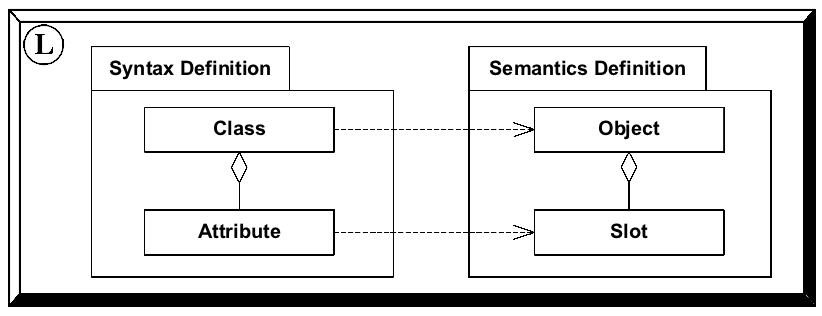
\includegraphics[width=0.9\textwidth]{dmm-metarelations.png}
    \caption{Пример вложенного соответствия}
    \label{fig4}
  \end{center}
\end{figure}

Семантической областью, т.е. системой, в терминах которой будет определяться семантика и выполняться интерпретация моделей, в DMM является технология преобразования графов, рассматриваемая далее. Семантика в данном подходе делится на статическую (static semantics) и динамическую (dynamic semantics). Статическая семантика на уровне языка представляет собой метамодель для описания набора состояний системы и доступных правил динамической операционной семантики без конкретной реализации. Семантическое соответствие синтаксической области на статическую семантику языка является денотационной частью DMM. Динамическая семантика на уровне языка является набором правил преобразований графов (graph transformation rules) и составляет операционную часть DMM.

В результате, на уровне модели в качестве реализации подходов, описанных на уровне языка, имеем систему LTS (meaning “LTS”), согласованную с ними, т.е. состояния (states) такой системы соответствуют состояниям, описанным в статической семантике на уровне языка. Правила перехода между этими состояниями являются правилами преобразования графов, которые реализованы на уровне языка, согласованы со статической семантикой и удовлетворяют синтаксическим особенностям создания правил, о которых будет рассказано в следующем параграфе.

\subsection{Преобразования графов}

В DMM модель, созданная на визуальном языке, рассматривается в виде типизированного мультиграфа с атрибутами и метками на узлах и рёбрах, допускающего наследование, связанного с возможностью расширения типов узлов и рёбер.

В общем виде, правило преобразования графов содержит левую и правую часть. Суть этих частей в следующем: в исходном графе ищется подграф, совпадающий с левой частью, и заменяется на граф из правой части. Для удобства левую и правую часть часто совмещают в одну, добавляя к каждому новому элементу метку \{new\}, а к каждому удалённому --- метку \{destroyed\}.

Такой поиск подграфа в графе модели очень похож на способ задания ограничений на данные в технологии REAL-IT~\cite{ivanov2}, формально описанный в работах А.Иванова~\cite{ivanov1, ivanov2, ivanov3}. Они позволяют в наглядном, графическом виде создавать ограничения на модель данных, заданную с помощью диаграмм сущность-связь. Например, часто может возникать ситуация, когда нельзя тот или иной объект соединить связью определённого типа с другим. Для таких случаев можно задать соответствующее ограничение, корректность которого будет впоследствии проверяться.

В DMM к этому описанию было добавлено несколько расширений: отрицающие применение условия (Negative Application Conditions, NAC) и универсальное замыкание (Universal Quantification, UQ). При использовании NAC к правилу добавляется несколько перечеркнутых элементов, означающих, что правило применимо только в случае отсутствия данных элементов в графе (правильным образом соединённых с остальными элементами искомого подграфа). Наличие же в правиле универсальной структуры (Universally Quantified Structures, UQS) означает, что правило будет применено сразу ко всем подходящим местам в исходном графе.

Для того, чтобы такие правила было удобно использовать, у каждого из них задаётся имя, список параметров и, по необходимости, ссылка на базовый элемент, для которого оно должно применяться. Это позволяет внутри одних правил вызывать для конкретных элементов другие (invocations).

На рис.~\ref{fig5} приведена общая сигнатура как правила (rule signature), так и вызовов других правил (invocation). Сигнатура правила состоит из четырёх частей: 
\begin{itemize}
 \item название правила (rule name);
 \item индикатор (big-step indicatior, “*”) того, что правило является правилом большого шага, которые могут применяться к исходному графу в любой момент, в отличие от правил малого шага, которые могут вызываться только внутри других правил;
 \item имя базового элемента (context node name, на рис.~\ref{fig5} это элемент “lman” типа ListManager, изображённый внутри правила в левой его части), для которого можно вызывать данное правило внутри других;
 \item список элементов-параметров (“parametername:type”, на рис.~\ref{fig5} это элемент “e” (signature parameter) типа Element).
\end{itemize}

\begin{figure} [ht]
  \begin{center}
    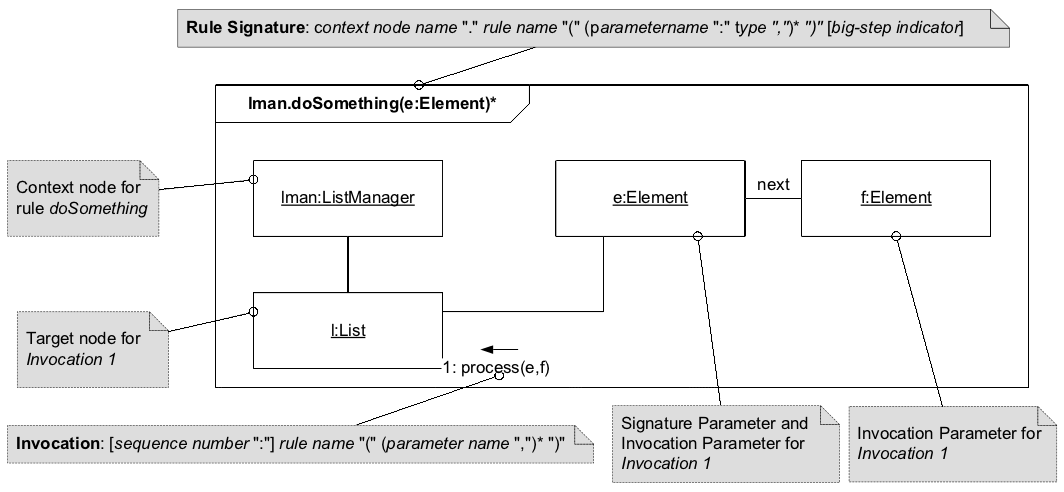
\includegraphics[width=1\textwidth]{dmm-signature.png}
    \caption{Сигнатура правила преобразования графов}
    \label{fig5}
  \end{center}
\end{figure}

Сигнатура вызова одного правила внутри другого состоит из трёх частей:
\begin{itemize}
 \item порядкового номера (sequence number), означающего порядок выполнения этих вызовов внутри данного правила;
 \item названия правила (rule name);
 \item списка элементов-параметров (“parametername:type”).
\end{itemize}

На рис.~\ref{fig5} приведён один такой вызов --- вызов правила process (“1:process(e, f)”). Такой вызов в этом правиле один, поэтому он имеет порядковый номер 1. Элемент (target node), для которого он вызывается, — элемент l типа List, параметры правила (invocation parameters) находятся по соответствующему имени.

\subsection{Примеры}

Рассмотрим несколько примеров использования DMM. На рис.~\ref{fig6}(а) изображено правило r1. Левая часть этого правила состоит из элементов типа Element и типа Buffer, правая --- из этих же элементов, только теперь они соединены связью. Данное правило ищет любую пару элементов типа Element и типа Buffer и добавляет между ними связь.

\begin{figure}[h]
\begin{minipage}[h]{0.49\linewidth}
\center{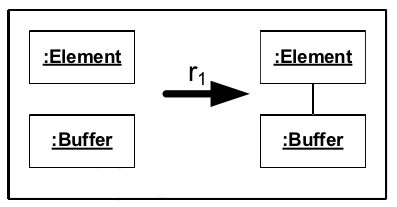
\includegraphics[width=1\linewidth]{dmm-nac-r1.png} \\ а)}
\end{minipage}
\begin{minipage}[h]{0.49\linewidth}
\center{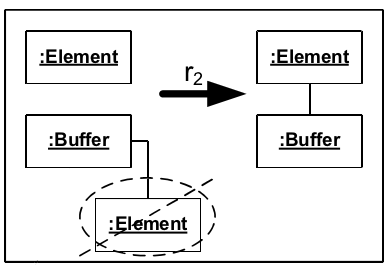
\includegraphics[width=1\linewidth]{dmm-nac-r2.png} \\ б)}
\end{minipage}
\begin{center}
\begin{minipage}[h]{0.49\linewidth}
\center{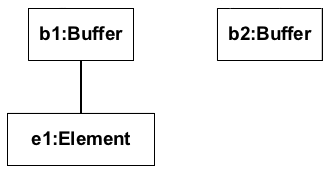
\includegraphics[width=1\linewidth]{dmm-nac-model.png} \\ в)}
\end{minipage}
\end{center}
\caption{а) --- правило r1 без использования NAC, б) — правило r2 с использованием NAC, в) — исходная модель}
\label{fig6}
\end{figure}

На рис.~\ref{fig6}(б) изображено правило r2, правая часть которого совпадает с правой частью правила r1, а левая часть содержит зачёркнутый элемент типа Element, связанный с элементом типа Buffer. Наличие такого перечёркнутого элемента и есть NAC для правила r2. Оно означает, что данное правило может быть применено к паре элементов типа Buffer и Element только при условии отсутствия связи элемента типа Buffer с произвольным элементом типа Element.

Модель на рис.~\ref{fig6}(в) состоит из двух буферов, один из которых связан с элементом типа Element. r1 может быть применено и к паре (b1, e1), и к паре (b2, e1), тогда как правило r2 --- только к паре (b2, e1).

На рис.~\ref{fig7}(а) показано, как при помощи UQS создать правило для полной очистки буфера. Данное правило называется flush и удаляет как все связи элемента типа Buffer с элементами типа Element, так и все эти элементы, т.к. в правой части они отсутствуют. Это достигается путём использования в правиле универсальной структуры. На это указывает двойная рамка у элемента с типом Element в левой части правила.

\begin{figure}[h]
\begin{center}
\begin{minipage}[h]{0.8\linewidth}
\center{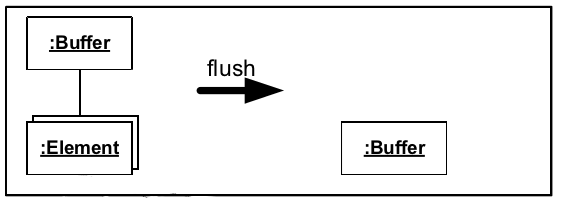
\includegraphics[width=0.8\linewidth]{dmm-uqs-flush.png} \\ а)}
\end{minipage}
\begin{minipage}[h]{0.8\linewidth}
\center{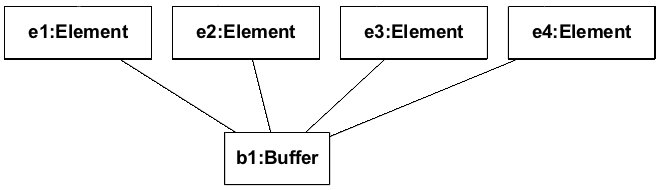
\includegraphics[width=0.8\linewidth]{dmm-uqs-model.png} \\ б)}
\end{minipage}
\end{center}
\caption{а) --- правило очистки буфера с использованием UQS, б) — исходная модель}
\label{fig7}
\end{figure}

Если применить данное правило к модели, изображённой на рис.~\ref{fig7}(б) и состоящей из буфера b1 и четырёх связанных с ним элементов, то элементы e1, e2, e3, e4 вместе со связями будут удалены и в модели останется один буфер.

В качестве примера вызова одного правила из другого рассмотрим следующую ситуацию. Есть набор списков, перечисляющих элементы Element типа ElementType, и сущность ListManager, которая ими управляет. Тип элемента и списка задаётся при помощи направленной связи с меткой type (на рис.~\ref{fig8}(а) она показывает тип списка и элемента new).

\begin{figure}[h]
\begin{center}
\begin{minipage}[h]{0.8\linewidth}
\center{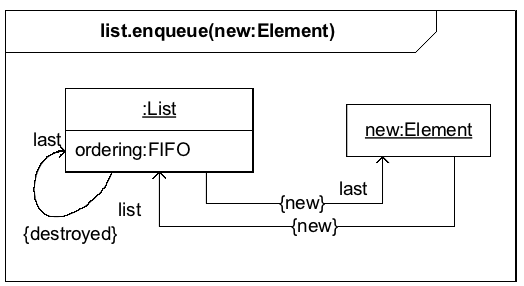
\includegraphics[width=0.8\linewidth]{dmm-enqueue.png} \\ а)}
\end{minipage}
\begin{minipage}[h]{0.8\linewidth}
\center{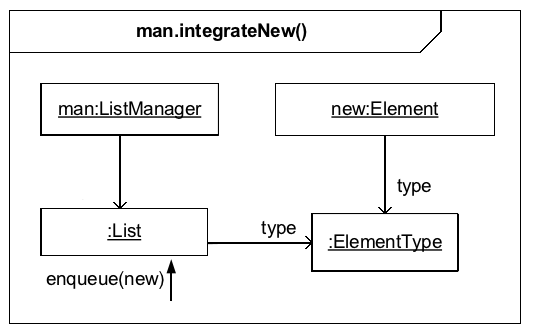
\includegraphics[width=0.8\linewidth]{dmm-integrateNew.png} \\ б)}
\end{minipage}
\end{center}
\caption{а) --- правило integrateNew, осуществляющее поиск нужного списка и вызов другого правила на нём, б) — правило enqueue со стратегией FIFO}
\label{fig8}
\end{figure}

Правило enqueue, непосредственно присоединяющее новый элемент к списку, может быть реализовано разными способами в зависимости от выбранной стратегии ипсользования списка (например, FIFO или LIFO). На рис.~\ref{fig8}(б) изображено правило enqueue, действуещее по стратегии FIFO. Оно также является правилом малого шага, может вызываться только на элементе типа List и принимает в качестве параметра элемент new типа Element. Для того, чтобы можно было использовать различные стратегии работы со списком, у элемента типа List есть атрибут ordering, который в этом случае предполагается равным FIFO. Как видно из рисунка, данное правило работает следующим образом: оно создаёт связь с меткой last между списком и элементом, тем самым показывая, что новый элемент стал последним в списке, добавляет обратную связь с меткой list между элементом и списком, по которой всегда можно найти, какому списку принадлежит элемент, а также удаляет старую связь с меткой last, зацикленную на самом списке, т.к. изначально список пуст.

\subsection{Анализ}

DMM-подход является зрелой технологией для задания семантики визуальных языков. Он формален, точен, универсален и понятен, имеет высокую наглядность как при задании семантики, так и при интерпретации моделей.

DMM потенциально можно использовать и для визуализации процесса отладки диаграмм. Можно организовать настраиваемое пошаговое исполнение, т.е. сколько правил следует применить перед следующим обновлением диаграммы, интерфейс, позволяющий следить за значениями атрибутов различных элементов и изменять их прямо во время исполнения и т.п. В случаях, когда правило можно применить в разных местах или когда есть несколько правил, которые можно применить на данном шаге, можно предоставлять этот выбор пользователю. Также можно ввести понятие точек останова, причём разных видов. Например, точка останова на применение конкретного правила, на изменение конкретного элемента, на получение определённой конструкции в графе модели и т.п. Подробнее с этими идеями можно ознакомиться в работе~\cite{dmm1}.

Среди главных недостатков этого подхода можно выделить высокую алгоритмическую сложность, связанную с задачей поиска подграфа в графе, которая является NP-полной, а также отсутствие реализации.

Если сравнивать DMM с xUML, то можно выделить следующие существенные отличия: DMM может применяться к любым визуальным языкам, а xUML фиксирован; семантика в DMM задаётся, в основном, визуально, а в xUML важную часть составляет код на AL; DMM подразумевает, что за ходом интерпретации можно будет наблюдать визуально, следя за изменениями модели, а для xUML эта визуализация будет состоять из подсветки текущего исполняемого элемента модели. 

\section{EProvide}

EProvide (Eclipse Plugin for Prototyping Visual Interpreters and Debuggers\footnote{EProvide, \url{eprovide.sourceforge.net}}) --- это подключаемый модуль (плагин) для среды разработки Eclipse\footnote{Eclipse, \url{www.eclipse.org}}, позволяющий быстро задавать операционную семантику для предметно-ориентированных языков, основанный на технологиях моделирования Eclipse~\cite{koznov7} (Eclipse Modeling Framework\footnote{EMF, \url{http://www.eclipse.org/modeling/emf}} (EMF), Graphical Modeling Framework\footnote{GMF, \url{http://www.eclipse.org/modeling/gmp}} (GMF)) и встраивающийся в систему исполнения программ Eclipse. Подход, использующийся в этом плагине, описан в статьях~\cite{wachsmuth1, wachsmuth2}.

\subsection{Описание подхода}

Обычно семантику языков моделирования записывают при помощи различных правил преобразования моделей, например, используя стандарт OMG Query/View/Transformation\footnote{QVT, \url{http://www.omg.org/spec/QVT}} (QVT). С их помощью можно переводить модели с одного языка на другой. Часто вторым языком является язык общего назначения, обладающий возможностью компиляции или интерпретации (например, Java, C++ или Python). Такой трансляционный подход в задании семантик уменьшает уровень абстракции, т.к. разработчику нужно разбираться сразу в двух предметных областях --- исходной и целевой, в которую происходит переход. Обеспечение обратной связи (например, в случае ошибок) целевой модели и исходной также является довольно сложной задачей. Такой подход является процедурой циклической разработки (round-trip engineering\footnote{\url{http://en.wikipedia.org/wiki/Round-trip_engineering}}~\cite{roundtrip}).

Весь набор способов задания семантики для произвольных языков можно разделить на несколько классов. Одним из основных классов является операционная семантика \footnote{\url{http://en.wikipedia.org/wiki/Operational_semantics}} (ОС). ОС языка представляет любой конкретный объект, записанный при помощи этого языка, в виде набора вычислительных шагов. Формально, её можно представить в виде пары $<\Gamma, \to>$, где $\Gamma$ --- множество конфигураций, а $\to$ — бинарное отношение перехода на множестве конфигураций. ОС бывают двух типов: структурная операционная семантика (СОС), предложенная Плоткиным~\cite{plotkin}, и естественная семантика.

Главным понятием в СОС является состояние. Обычно это набор определённых переменных и их значений. Конфигурацией же является пара $<S, \sigma>$, где S --- фрагмент программы, а $\sigma$  — текущее состояние. Отношение перехода также является бинарным отношением на множестве конфигураций. Таким образом, переходы в СОС описываются согласно абстрактным синтаксическим конструкциям языка, появляется возможность задавать для языков абстрактные интерпретаторы, основанные на их синтаксисе. Также СОС позволяет использовать структурную индукцию, например, при доказательстве корректности интерпретаторов и отладчиков.

Ваксмут (Wachsmuth) предложил использовать СОС, записанную декларативным текстовым способом при помощи языка QVT Relations~\cite{qvt}, являющегося частью стандарта OMG QVT. QVT Relations --- это высокоуровневый декларативный язык, разработанный для создания как односторонних, так и двухсторонних преобразований моделей. Позже в работе~\cite{wachsmuth1} этот подход был совмещён с технологиями визуального моделирования, и был реализован подключаемый модуль EProvide, позволяющий прототипировать визуальные интерпретаторы и отладчики для предметных языков. Также были добавлены и другие языки для описания семантики: Java, Abstract State Machines~\cite{asm} (ASM), Prolog и Scheme\footnote{Scheme, \url{http://www.r6rs.org}}.

Важно отметить, что при интерпретации или отладке происходит изменение состояния модели, которое, во-первых, нужно возвращать к исходному состоянию в конце интерпретации или при ручной остановке, а во-вторых, это состояние нужно уметь изменять в режиме отладки через графический интерфейс пользователя. Для этого необходимо вручную создать отдельную от исходной метамодель, состояние экземпляров элементов которой и будет изменяться. Также туда можно добавить дополнительные структуры, необходимые, например, для обеспечения функциональности точек останова. Рассмотрим предлагаемый подход более подробно на примере сетей Петри.

\subsection{Редактор и семантика для сетей Петри в EProvide}

Сети Петри в простейшем случае можно представить в виде набора позиций с некоторым числом меток (токенов) и переходов, которые могут иметь имена. У перехода может быть набор входящих и исходящих позиций.

На рис.~\ref{fig9}(а) изображена метамодель для сетей Петри с двумя элементами: позиция и переход. Сеть (Net) содержит в себе произвольное количество переходов (Transition) и позиций (Place). У перехода и позиции могут быть имена, поэтому соответствующие элементы содержат атрибут name. В сетях Петри у позиции может быть некоторое число токенов, количество которых хранится в атрибуте token, на которое наложено ограничение неотрицательности. Переходы же содержат наборы входящих (src) в и исходящих (snk) из него позиций.

\begin{figure}[h]
\begin{center}
\begin{minipage}[h]{0.8\linewidth}
\center{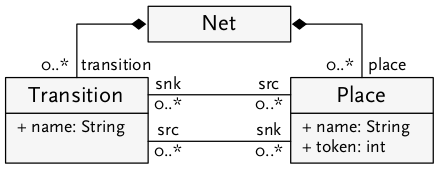
\includegraphics[width=0.8\linewidth]{eprovide-petrinet-model.png} \\ а)}
\end{minipage}
\begin{minipage}[h]{0.8\linewidth}
\center{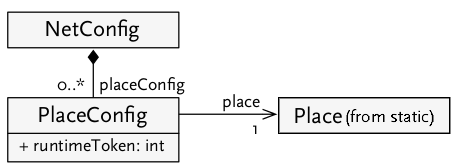
\includegraphics[width=0.8\linewidth]{eprovide-petrinet-additionalmodel.png} \\ б)}
\end{minipage}
\end{center}
\caption{а) --- общая метамодель сетей Петри (этот рисунок и все последующие в этом разделе взяты из работы~\cite{wachsmuth1}), б) — метамодель времени исполнения для сетей Петри}
\label{fig9}
\end{figure}

На рис.~\ref{fig9}(б) находится расширение общей метамодели для хранения состояний элементов в период исполнения. Конфигурируемая сеть (NetConfig) содержит в себе некоторое число (совпадающее с числом позиций в исходной сети) конфигурируемых позиций (PlaceConfig). Каждой такой позиции соответствует одна и ровно одна позиция из статической метамодели, и изменения происходят только с ней, т.е. во время исполнения она содержит в атрибуте runtimeToken текущее количество токенов в исходной позиции.

В качестве примера на рис.~\ref{fig10} изображён фрагмент семантики сетей Петри, заданный с помощью QVT Relations. Для этого определено преобразование (transformation) petri\_sos, имеющее в качестве своих областей входных (input) и выходных (output) значений модели сетей Петри.

\begin{figure} [ht]
  \begin{center}
    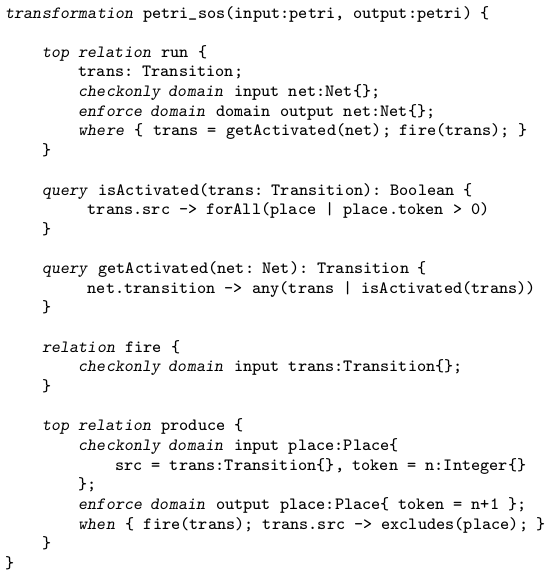
\includegraphics[width=0.7\textwidth]{eprovide-petrinet-qvt.png}
    \caption{Фрагмент семантики сетей Петри, записанный при помощи QVT Relations}
    \label{fig10}
  \end{center}
\end{figure}

Любое преобразование в QVT Relations состоит из запросов (queries) и отношений (relations). Запрос в отличие от отношения возвращает результат некоторого OCL выражения~\cite{ocl}. В задании семантики сетей Петри используется два вида запросов: isActivated, проверяющий, может ли сработать переход или нет, и getActivated, возвращающий переход, который может. isActivated возвращает булевское значение и имеет своим аргументом некоторый переход trans. У этого перехода берутся все входящие в него позиции (trans.src) и с помощью цикла forAll проверяется, что число токенов в них положительно. getActivated в качестве параметра принимает всю сеть (net) и возвращает некоторый элемент типа Transition. У сети берутся все переходы (net.transition) и при помощи OCL предиката any возвращается произвольный переход, удовлетворяющий условию isActivated, т.е. первый переход, который может сработать.

Отношения определяют новые области (domains) и переменные и позволяют производить некоторые операции над самой моделью. Отношение, объявленное с идентификатором top, будет применено (hold) для успешного проведения процедуры преобразования целиком. Если нет, то отношение производит преобразования над элементами выходной модели, объявленные при помощи идентификатора enforce. Также отношение может содержать where- или when- блоки.  Where-блок позволяет устанавливать дополнительные ограничения в отношении используемых элементов, при чём у этих ограничений может быть идентификатор enforce. When-блок же определяет дополнительные условия на применение отношения. Отношения без идентификатора top могут быть применены только внутри where-блока другого отношения.

Как видно из рис.~\ref{fig10}, в семантике присутствует одно отношение fire, не объявленное, как top. Оно проверяет, присутствует ли переход во входной модели. Отношение run определяет две области. Первую, содержащуюся в input и являющуюся моделью сети Петри, оно связывает с переменной net. Вторую же, содержащуюся в output, оно насильно (enforce) связывает с переменной net, показывая таким образом, что результат всех операций, производимых над входной моделью, в ней же и останется. В where-блоке отношение run берёт переход, который может сработать, и применяет к нему fire. Таким образом, отношение run может быть применено тогда и только тогда, когда в модели сети Петри есть переход, который может сработать.

Отношения produce, consume и preserve продолжают начатую с run активацию перехода и соответствуют ситуациям, когда у позиции нужно изменить число токенов (то есть для тех позиций, которые непосредственно связаны с сработавшим переходом): увеличить или уменьшить на 1, оставить неизменённым.

Разберём подробнее отношение produce. Оно также, как и run, объявлено top-отношением. В качестве входных данных оно берёт позицию place из области input, обозначает переход (src), из которого в неё можно перейти, за trans, а число токенов в ней за n. После этого в выходной области output, т.е., как было замечено ранее, в той же самой, оно увеличивает число токенов у place на 1. Применено же оно может быть только, если на trans сработало отношение fire и если place не является входной позицией для trans.

Данный набор правил при использовании будет изменять исходную модель сети Петри, а не модель времени исполнения, поэтому нужно добавить в него пару правил, её инициализирующих. Также можно расширить метамодель времени исполнения точками останова и добавить соответствующих правил в семантику для обеспечения их поддержки (в данной статье не рассматривается). Подробнее ознакомиться с тем, как создать полноценный отлаживаемый исполняемый визуальный язык для сетей Петри при помощи EProvide, можно в статье~\cite{wachsmuth1}.

Все метамодели, используемые в EProvide, согласованы со стандартом MOF~\cite{mof} и работа с ними на уровне редактора моделей осуществляется при помощи технологий EMF и GMF. Это включает в себя, например, изменение значений атрибутов модели времени исполнения при интерпретации и подсветку различных элементов при необходимости. Модуль, отвечающий за правильное применение преобразований QVT Realations, написан авторами статьи самостоятельно. 

Также была разрешена следующая проблема. GMF не поддерживает то расширение редакторов, которое необходимо для организации моделей времени исполнения, т.к. для этого нужно расширить множество элементов логического представления (добавить PlaceConfig) и сделать ссылку на графическое представление Place для PlaceConfig. Поэтому в EProvide создаётся объединённая метамодель. Для этого в сущность Net добавляется атрибут running, сигнализирующий о том, симулируется ли сейчас данная сеть или нет, а в сущность Place добавляются initToken (начальное значение) и runtimeToken (текущее значение при симуляции). Исходный атрибут token теперь просто ссылается на initToken или runtimeToken в зависимости от значения Net.running.

Как видно из рис.~\ref{fig11}, EProvide позволяет изменять состояние элементов модели прямо в процессе отладки (окно слева), подсвечивает сработавший переход, отображает состояние модели времени исполнения, а не исходной. В конце интерпретации или при ручной остановке модель возвращается в исходное состояние. Это происходит автоматически вследствие разделения на исходную статическую модель и модель времени исполнения, отображаемую пользователю.

\begin{figure} [ht]
  \begin{center}
    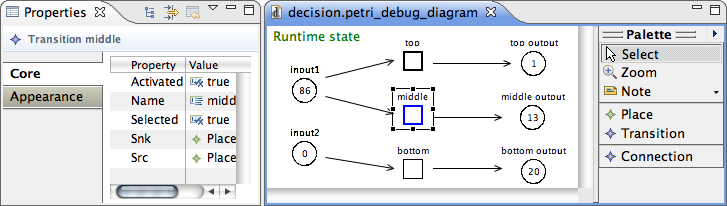
\includegraphics[width=0.9\textwidth]{eprovide-screen.png}
    \caption{Графический интерфейс отладчика для сетей Петри}
    \label{fig11}
  \end{center}
\end{figure}

\subsection{Анализ}

Подход, предложенный Ваксмутом, является достаточно общим и позволяет работать с различными языками спецификаций, с помощью которых будет происходить непосредственное задание семантики, имеет гибкую позицию относительно реализации точек останова и прочих функциональностей стандартных отладчиков, полноценно реализован под платформу Eclipse. Но если смотреть со стороны удобства использования, то ручное написание семантики на каком-либо текстовом языке понижает достигнутый уровень абстракции. И для успешного применения этого подхода в средах, отличных от Eclipse, необходимо наличие интерпретатора данного языка, реализация которого может оказаться нетривиальной задачей.

От xUML EProvide отличается тем, что для задания семантики достаточно лишь описать метамодель языка и способ трансформации моделей, например, при помощи стандарта QVT Relations, и не нужно рисовать много UML диаграмм. В EProvide легко можно организовать пошаговое исполнение, совмещённое с поддержкой различного вида точек останова и слежения за значениями атрибутов элементов. Для xUML, как было отмечено в параграфе 3.2, существует множество поддерживающих его программных средств, что усложняет выбор среди них при необходимости решить определённую задачу.

DMM, так же как и EProvide, основан на преобразованиях моделей. Но в отличие от EProvide способ задания семантики в нём более естественен, т.к. является визуальным. К тому же он основан на хорошо исследованной области преобразования графов, что способствует, например, доказуемости поведения программ. DMM имеет пару особенностей, взятых из формальной теории преобразования графов, например, NAC и UQS, а EProvide зато поддерживает более обширный функционал для задания ограничений на применение своих правил (отношений) при помощи when- и where- блоков, а также позволяет осуществлять различные запросы на входной модели, удобство использования этой функциональности было продемонстрировано на примере сетей Петри.

\section*{Дискуссия и заключение}

Предметно-ориентированное моделирование при определенных условиях может довольно сильно повышать производительность труда разработчиков. Одним из таких условий является адекватная инструментальная поддержка, в которую входит довольно большой набор средств, начиная от визуального редактора и репозитория и заканчивая средствами отладки, версионирования или рефакторингов создаваемых моделей. Для эффективной поддержки предметно-ориетированной парадигмы DSM-платформы должны обладать средствами автоматизированного создания всех необходимых инструментов, ручное кодирование даже хотя бы одного инструмента делает данный подход к разработке ПО неприменимым.

Традиционно создание нового языка начинается с анализа предметной области и выделения в ней сущностей и связей между ними, важных для решаемой задачи. Эти сущности фиксируются в элементах языка и их свойствах, связи между сущностями --- в отношениях и ассоциациях. Для графических языков эта информация чаще всего задается в виде метамодели (модели абстрактного синтаксиса языка) и является достаточной для того, чтобы автоматизированно получить работающий редактор визуальных моделей. Метамодель задает правила формирования конструкций из элементов языка, но никак не объясняет, что эти элементы и конструкции значат — не задает семантику языка. Для многих языков моделирования семантика определяется неформально с помощью описаний на естественном языке (русском, английском или любом другом), подкрепленных примерами использования. И если для языков моделирования (как, например, UML) это вполне приемлемо, то для языков программирования наличие формально заданной семантической модели является ключевым фактором 
исполнимости программ, созданных с помощью данного языка. Отсутствие формально заданной семантики приводит к неоднозначности трактования моделей на этом языке, что делает автоматизированное построение и использование генераторов, интерпретаторов и отладчиков моделей практически невозможным. 

В статье были рассмотрены существующие подходы к описанию исполнимой семантики, выделены и описаны некоторые основные методы по заданию семантики визуальных языков. 

На основе анализа данных методов можно предложить следующий подход, сочетающий в себе их лучшие стороны. В качестве графической составляющей задания семантики можно использовать технологию преобразования графов, описанную в DMM. Дополнительные ограничения на применение правил можно записывать при помощи OCL, о котором упоминается в EProvide. Для визуализации потока исполнения можно ввести специальный маркер, являющийся отдельным графическим элементом семантики. Связь с ним означала бы подсветку соответствующего элемента интерпретируемой модели (либо любое другой действие, отличающие текущий исполняемый элемент модели от других).

Из семантики xUML можно взять её текстовую составляющую. А именно, задание возможного поведения объектов в целом, а также при проходе каждого состояния в диаграмме состояний при помощи AL. Для этого можно ввести понятие реакции на применение правила, которую можно задавать либо на AL, либо на другом интерпретируемом текстовом языке, обеспечивающем взаимодействие между элементами правила, изменение их атрибутов и т.п.

Сложность реализации данного подхода зависит от платформы, на которой его нужно реализовать. Наиболее существенная и сложная часть в реализации --- это модуль, отвечающий за организацию преобразований графов. При использовании java-технологий для этого можно воспользоваться готовыми средствами AGG~\cite{agg} или GROOVE~\cite{groove}, однако конвертацию исходной визуальной модели в формат, поддерживаемый данными продуктами, нужно реализовывать самостоятельно. Для вычисления OCL-выражений можно воспользоваться средством USE\footnote{USE, http://sourceforge.net/apps/mediawiki/useocl}.

\begin{thebibliography}{9001}
\bibitem{unimod} \emph{Гуров В., Мазин М., Шалыто А.} UniMod - инструментальное средство для автоматного программирования // Научно-технический вестник информационных технологий, механики и оптики. 2006. № 30. С. 32-45.
\bibitem{ivanov1} \emph{Иванов А.} Графический язык описания ограничений на диаграммы классов UML // Программирование. 2004. No 4. С. 204–208.
\bibitem{ivanov2} \emph{Иванов А.} Технологическое решение REAL-IT: создание информационных систем на основе визуального моделирования // Системное программирование. Под ред. А. Н. Терехова, Д. Ю. Булычева. Изд-во СПбГУ, 2004. С. 89–100.
\bibitem{ivanov3} \emph{Иванов А., Стригун С.} Технологическое решение REAL-IT: автоматизированная разработка пользовательского интерфейса информационных систем // Системное программирование. Под ред. А. Н. Терехова, Д. Ю. Булычева. Изд-во СПбГУ, 2004. С. 124-147.
\bibitem{kartashev} \emph{Карташев М.} Двухуровневая схема отладки // Системное программирование. Под ред. А. Н. Терехова, Д. Ю. Булычева. Изд-во СПбГУ, 2004. С. 348-365.
\bibitem{koznov1} \emph{Кознов Д.В.} Визуальное моделирование компонентного программного обеспечения.  Автореферат диссертации на соискание ученой степени кандидата физико-математических наук. Санкт-Петербург. 2000.
\bibitem{koznov2} \emph{Кознов Д.В.} Разработка и сопровождение DSM-решений на основе MSF // Системное программирование. Под ред. А. Н. Терехова, Д. Ю. Булычева. Изд-во СПбГУ, 2008. Т. 3. № 1. С. 80-96.
\bibitem{koznov3} \emph{Кознов Д.В., Иванов А.Н.} Поддержка концептуального моделирования при разработке визуальных языков с использованием Microsoft DSL Tools // Системное программирование. Под ред. А. Н. Терехова, Д. Ю. Булычева. Изд-во СПбГУ, 2009. Т. 4. С. 105-127.
\bibitem{koznov4} \emph{Кознов Д.В., Ольхович Л.Б.} Визуальные языки проектов // Системное программирование. Под ред. А. Н. Терехова, Д. Ю. Булычева. Изд-во СПбГУ, 2005. Т.1. № 0. С. 148-167.
\bibitem{koznov5} \emph{Павлинов А., Кознов Д., Перегудов А., Бугайченко Д., Казакова А., Чернятчик Р., Фесенко Т., Иванов А.} Комплекс средств разработки проблемно-ориентированных визуальных языков // Вестник Санкт-Петербургского университета. Серия 10: Прикладная математика. Информатика. Процессы управления. 2007. № 2. С. 86.
\bibitem{koznov6} \emph{Павлинов А., Кознов Д., Перегудов А. и др.} О средствах разработки проблемно-ориентированных визуальных языков // Системное программирование / Вып. 2, под ред. А. Н. Терехова и Д. Ю. Булычева. СПб.: Изд. СПбГУ, 2006. С. 116-141.
\bibitem{koznov7} \emph{Сорокин А., Кознов Д.} Обзор Eclipse Modeling Project // Системное программирование / Вып. 5, под ред. А. Н. Терехова и Д. Ю. Булычева. СПб.: Изд. СПбГУ, 2010. С. 6-31.
\bibitem{dmm1} \emph{Bandener N.} Visual interpreter and debugger for dynamic models based on the Eclipse platform. Diploma Thesis, 2009, Faculty of Computer Science, Electrical Engineering, and Mathematics of the University of Paderborn. 125 p.
\bibitem{asm} \emph{Borger E., Stark R.} Abstract State Machines: A Method for High-Level System Design and Analysis // Springer-Verlag, 2003. 35 p.
\bibitem{xuml1} \emph{Boyd G.} Executable UML: Diagrams for the Future. 2003. \url{http://www.devx.com/enterprise/Article/10717}
\bibitem{dmm2} \emph{Hausmann J.} Dynamic Meta Modeling: A Semantics Description Technique for Visual Modeling Languages. PhD Thesis, 2005, Paderborn, Faculty of Computer Science, Electrical Engineering, and Mathematics of the University of Paderborn. 326 p.
\bibitem{hoare} \emph{Hoare C.A.R.} An axiomatic basis for computer programming // Communications of the ACM, 12(10):576–580, 1969, P. 576-583.
\bibitem{semantics1} \emph{Kahn G.} Natural Semantics // Proceedings of the 4th Annual Symposium on Theoretical Aspects of Computer Science, Springer-Verlag, London, 1987, P. 22-39.
\bibitem{dsmbook} \emph{Kelly S., Tolvanen J.} Domain-Specific Modeling: Enabling Full Code Generation // Wiley-IEEE Computer Society Press, 2008. 448 p.
\bibitem{xuml2} \emph{Mathew A.} Software Development Using Executable UML (xUML). 2002. \url{http://se.cs.depaul.edu/ise/zoom/projects/statechart/SE690DetailedPresentation.ppt}
\bibitem{xuml3} \emph{Mellor S., Balcer M.} Executable UML: A foundation for model-driven architecture // Addison Wesley, 2002. 416 p.
\bibitem{mof} Meta Object Facility (MOF) 2.0 Core Specification. OMG. 2006.
\bibitem{qvt} Meta Object Facility (MOF) 2.0 Query/View/Transformation Specification. Version 1.0. OMG. 2008.
\bibitem{oal} Object Action Language Reference Manual. 2008. 77 p. \url{www.ooatool.com/docs/OAL08.pdf}
\bibitem{uml} OMG Unified Modeling Language, Superstructure. Version 2.4.1. OMG. 2011. 732 p.
\bibitem{plotkin} \emph{Plotkin G.} A Structural Approach to Operational Semantics // Technical Report DAIMI FN-19, University of Aarhus, 1981. 133 p.
\bibitem{groove} \emph{Rensink A.} The GROOVE Simulator: A Tool for State Space Generation // AGTIVE 2003 – Revised   Selected and Invited Papers, volume 3062 of Lecture Notes in Computer Science, Berlin, Springer Verlag, 2004, P. 479–485.
\bibitem{wachsmuth1} \emph{Sadilek D., Wachsmuth G.} Prototyping Visual Interpreters and Debuggers for Domain-Specific Modelling Languages // ECMDA-FA 2008, LNCS 5095, 2008, P. 64–79.
\bibitem{semantics2} \emph{Scott D., Strachey C.} Towards a Mathematical Semantics for Computer Languages // Computers and Automata, Wiley, 1971, P. 19–46.
\bibitem{roundtrip} \emph{Sendall S., Kuster J.} Taming Model Round-Trip Engineering // Proc. Workshop on Best Practices for Model-Driven Software Development (part of 19th Annual ACM Conference on Object-Oriented Programming , Systems, Languages, Applications). 2004. 13 p.
\bibitem{al1} Shlaer-Mellor Action Language. 1997. 29 p. \url{www.modelint.com/downloads/small.pdf}
\bibitem{translational} \emph{Slonneger K., Kurtz B.} Syntax and Semantics of Programming Languages, A Laboratory Based Approach // Addison-Wesley Publishing, 1995. P.187-222.
\bibitem{agg} \emph{Taentzer G.} AGG: A graph transformation environment for system modeling and validation // Proc. Tool Exihibition at Formal Methods’03, 2003. 9 p.
\bibitem{wachsmuth2} \emph{Wachsmuth G.} Modelling the Operational Semantics of Domain-Specific Modelling Languages // Generative and Transformational Techniques in Software Engineering II. Lecture Notes in Computer Science Volume 5235, Springer, 2008, P. 506-520.
\bibitem{ocl} \emph{Warmer J., Kleppe A.} The Object Constraint Language: Precise Modeling with UML // Addison- Wesley Object Technology Services, Reading, MA, 1999. 144 p.
\bibitem{xuml4} \emph{Wilkie I.} Executable UML and SPARK Ada: The Best of Both Worlds // Kennedy Carter Ltd, 2006. 6 p.
\bibitem{al2} \emph{Wilkie I. et al.} The Action Specification Language Reference Manual // Kennedy Carter Ltd, 2003. 112 p.
\end{thebibliography}

\end{document}
